\section{Results}
In the interest of consolidating operators it is critical to find an accurate measurement that detects situations that exceed the capacity of a given human. One way to detect this is by building a map of each actor's workload as a function of time. JPF explores all possible paths the model can take and returns the ones that violate the model's criteria. By augmenting our model with the workload metrics we can identify all possible areas of high workload. 

We propose three levels of increasing validity for evaluating the approach in the paper.  The first level, the one used in this paper, is to check for {\em consistency}.  We say that the approach is {\em consistent} if the workload peaks, valleys, and trends match what we know about a small set of given situations; in other words, the approach is consistent if it matches our expectations on tasks that we know a lot about.  

The second level, which is an area for future work, is to check for {\em sensitivity}.  We say that  the approach is sufficiently {\em sensitive} if we can use JPF to find new scenarios that have very high or very low workloads, and we can then generate a satisfactory explanation for the levels of workload by evaluating the new scenarios.  The third level, another area of future work, is to {\em substantiate} workload levels using experiments with human participants by comparing the perceived workload of humans with those predicted by the model.

In this paper, we restrict attention to finding areas of high and low workload, and then checking these areas for consistency.  We evaluated consistency using two scenarios.  The first is when the Video Operator was able to identify the target during a flight without any complications occurring (see Figure~\ref{fig:WorkloadSim1}). As the workload measure currently does not have units, the plots are normalized in each category. For the first 40 time steps everything behaves as expected with low to moderate workload. An initial workload bump occurs as actors exchange information necessary to start a search.   At time step forty we see a dramatic deviation from the norm. This deviation is a result of constant information passing between the GUIs and the operators
making it only
%. Since there is a constant passing of data between the machinery and the operators, it is only
 logical that the workload would increase substantially.

\begin{figure}[h]
\center
\setlength{\abovecaptionskip}{1mm}
\setlength{\belowcaptionskip}{1mm}
\setlength{\textfloatsep}{1mm}
\setlength{\floatsep}{1mm}
\scalebox{.9}{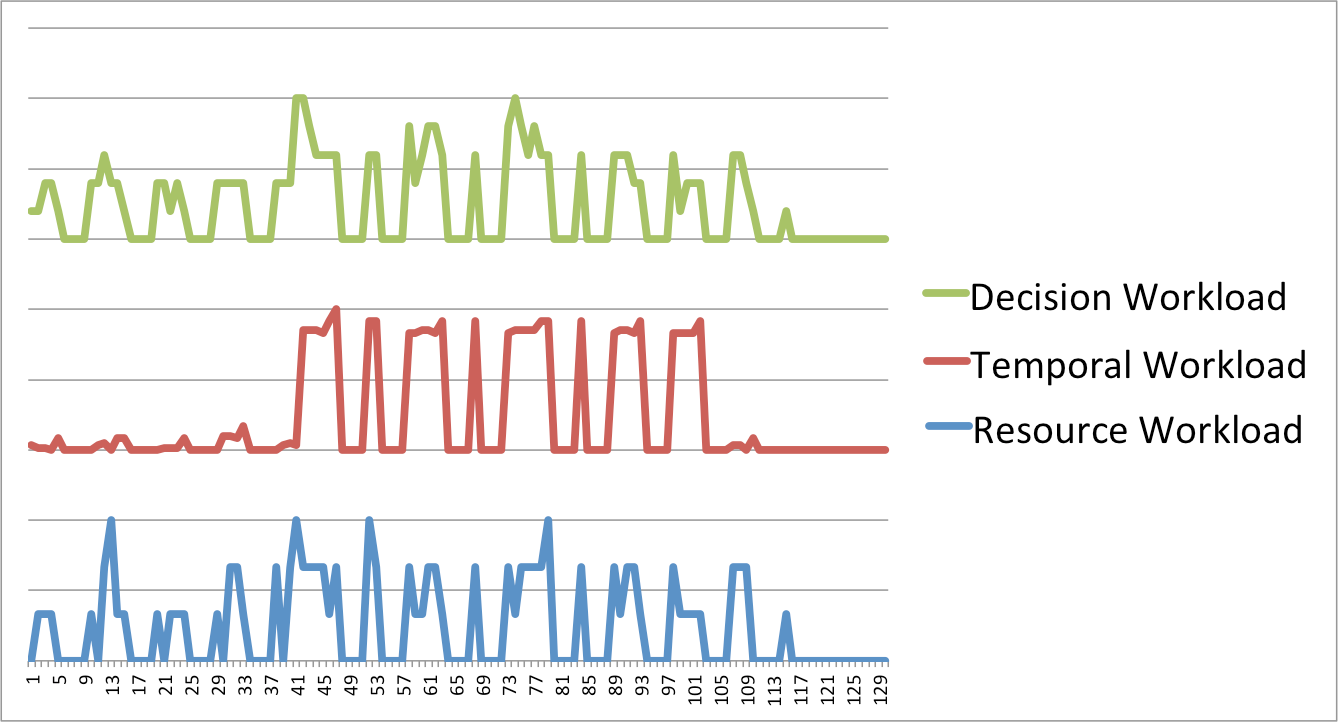
\includegraphics[height=2in]{WorkloadTargetSightingLabeled.png}}
\caption{Workload over an uneventful flight.}
\label{fig:WorkloadSim1}
\end{figure}

The second simulation is a scenario where after a short period of flight the battery rapidly fails. In this particular situation, the operator was unable to respond quickly enough to land the UAV before it crashed (see Figure~\ref{fig:WorkloadSim2}). There is an immediate spike in the temporal workload (middle plot), but surprisingly, the workload then decreases back to normal levels in just five time steps. The second spike indicates an unexpected fluctuation in options among one of the actors, which will have to be investigated further to verify if this is an accurate response or if a flaw in the model had slipped past the verification stage of development. Finally, as would be expected, when the UAV crashed there was a small spike in the workload before everything came to a halt. 

\begin{figure}[h]
\center
\setlength{\abovecaptionskip}{1mm}
\setlength{\belowcaptionskip}{1mm}
\setlength{\textfloatsep}{1mm}
\setlength{\floatsep}{1mm}
\scalebox{.75}{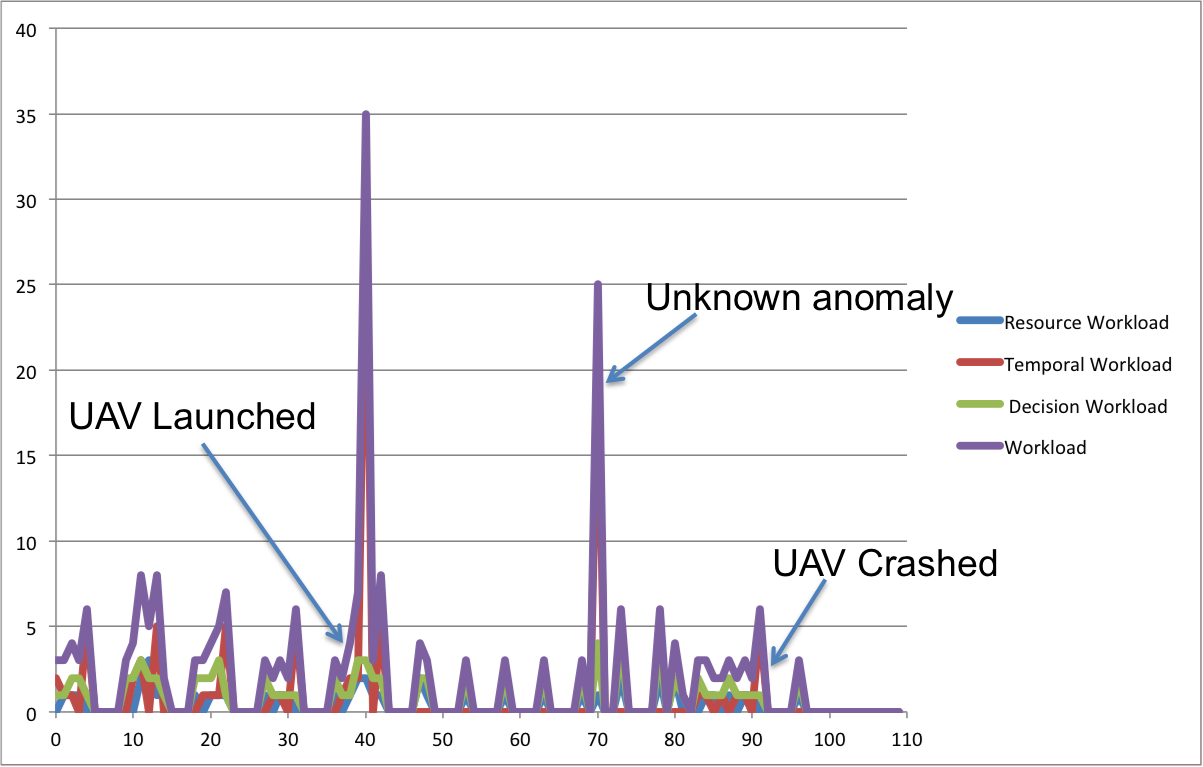
\includegraphics[height=2in]{WorkloadCrashedLabeled.png}}
\caption{Emergency battery failure simulation}
\label{fig:WorkloadSim2}
\end{figure}
